\chapter{種々の函数}

\begin{flushright}
担当教員: 植野 義明 / TA: 穂坂 秀昭 \\
講義日時: 2015年4月22日 1限
\end{flushright}

\section{全体的な講評}

今回のテーマは「高校生のうちに一応習いはするけど、でもあんまり深入りはしない函数たち」です。逆三角函数や双曲線函数について、名前自体は授業前から知っていた人が多かったのではないでしょうか。いずれの問題も、そうした函数の性質を知るためのものです。

問題は比較的易しいものが多かったので、ほとんどの人が良く解けていました。中には一つの問題に複数の方法で取り組んだり、あるいは関連する問題をまとめて解いたりした人がいました。大変良いことだと思います。普通に問題を解くのに加え、問題を解く過程から何かを見出せるよう頑張ってください。

また今回、答案の中に質問やリクエストを書いてくれた人もいました。そういうことが書いてあると解説プリントを作るときの指針になりますので、何か思うことがあれば、ぜひ答案内に書き込んでおいてください。

それでは、今回のテーマを一つずつ見ていきましょう。

\section{逆函数について}


\subsection{逆函数の定義}

函数とは、数に対して何かしらの数を対応させる規則のことです。たとえば$f(x)=x^2$という函数は、実数$x\in\mathbb{R}$に$x^2\in\mathbb{R}$という数を対応させています。他にも三角函数、対数函数や指数函数といった有名な函数があり、そしてこれらの函数を合成するとさらに色々な函数を作ることができますが、どの函数も\textbf{数に数を対応させる}ことには間違いありません。別の言い方をすれば、僕たちが普段「函数」と呼んでいるものは、定義域と値域が実数全体$\mathbb{R}$ (の部分集合) であるような写像です\footnote{ただし、この用語の使い方は慣用的なもので、厳密な取り決めがあるわけではありません。たとえば定義域や値域がベクトルの集合であっても、函数と呼ぶことはままあります。}。

さて函数$f(x)$が与えられると、数$x$が与えられた時に$f$の値$f(x)$が定まります。そしてしばしば「数$y$が与えられたとき、$y=f(x)$となる数$x$を求めたい」という状況が生じます。対応$x\mapsto f(x)$ではなく、その逆の対応を求めたいわけです。このように函数$f$が与えられたとき、「数$y$に対し、$y=f(x)$となる$x$を対応させる」という方法で定義される函数を$f$の\textbf{逆函数}と言い、$f^{-1}$と書きます。$x\mapsto f(x)$の対応が逆になるので、逆函数のグラフは元の函数のグラフを直線$y=x$について線対称に折り返したものになります。

\subsection{逆函数の主値}

\paragraph{逆函数を定義するための条件} 残念なことに、与えられた函数に対していつでも逆函数が無条件で定義できるわけではありません。上で述べたように、函数は写像ですから「$1$つの数に、$1$つの数を対応させる」ことが大原則です。だから「$1$つの数に$2$つの数を対応させる」という操作になってしまっては、函数とは呼べないのです。

いま、函数$f$が相異なる実数$x_1$, $x_2$に対して$f(x_1)=f(x_2)$を満たしたとしましょう。そして$y=f(x_1)=f(x_2)$とおきます。すると$x_1$, $x_2$のどちらに対しても$y$が対応するので、逆函数を作ろうとしたら「$y$に$x_1$, $x_2$の両方が対応する」というマズい状況が実際に起きます。こうならないためには「異なる実数$x_1$, $x_2$に対して必ず$f(x_1)\neq f(x_2)$が成り立つ」という条件が必要です。こういう性質を$\textbf{単射性}$というのでした。

また単射なら良いかというと、そうでもありません。たとえば指数函数$\exp x:=e^x$を考えましょう。指数函数を$\exp\colon \mathbb{R}\rightarrow\mathbb{R}$という写像と思えば、これは単射です。グラフを描けば狭義短調増加ですから、異なる値に対して同じ値が対応しようがありません。そして正の実数$y>0$に対しては、$e^x = y$となる$x$が$x=\log y$で与えられます。ですが$y\leq 0$のとき、$y=\exp x$となる$x\in\mathbb{R}$は存在しません。さっきは「$1$つの数に$2$個 (以上) の数が対応してしまう」ことが問題でしたが、今度は「ある数に対して、対応させられる数がなくなってしまった」という問題が起きています。これももちろん写像の定義を満たさないので、指数函数$\exp$を$\mathbb{R}$から$\mathbb{R}$への写像と思うと、逆函数は作れません。ですが$\exp$の値域を正の整数全体の集合$\mathbb{R}_{>0}:=\{x\in\mathbb{R} \mid x>0 \}$だと思えば、どんな正の数$y>0$に対しても$x:=\log y$とおくことで$y=e^x$なる実数$x$を見つけられます。このような、函数$f$の「どんな値域の元$y$に対しても、$y=f(x)$となる$x$が存在する」という性質を、\textbf{全射性}と呼ぶのでした。

まとめると、\textbf{$f$の逆函数が存在するための必要条件は、$f$が全単射であること}です。また$f$の逆函数$g$が存在すれば、$f$は全単射になると示せます。かくして$f$の逆函数が存在することと、$f$が全単射であることが同値だと分かります。

\paragraph{逆函数の主値}

ただし$f$が全単射でないときも、部分的には$f$の逆函数を作れることが多いです。さっきの指数函数の例では、値域を$\mathbb{R}$から$\mathbb{R}_{>0}$に取り換えれば逆函数が作れました。また$f$の定義域を制限してしまうのも一つの手です。たとえば$f(x)=x^2$という函数を考えましょう。正の実数$x>0$に対し$f(-x)=(-x)^2=x^2=f(x)$という式が成り立ってしまうので、$f$は単射ではありません。ですが$f$の定義域を非負実数全体の集合$\mathbb{R}_{\geq 0}:=\{x\in\mathbb{R}\mid x\geq 0\}$に制限してしまえば、$f$は単射になります。そしてどんな非負の実数$y\in\mathbb{R}_{\geq 0}$に対しても、$x:=\sqrt{y}$とおけば$y=x^2=f(x)$が成り立ちます。こうして$f$を制限して$\mathbb{R}_{\geq 0}\rightarrow\mathbb{R}_{\geq 0}$という写像にすれば、$f$の逆函数$y\mapsto \sqrt{y}$が得られます。$f$の定義域を制限して逆写像$f^{-1}$を作るとき、その値を$f^{-1}$の\textbf{主値}と言います。

ちなみに複素数の偏角$\arg$の「主値」という言葉遣いも、函数の主値と同じ意味です。$0$以外の複素数全体の集合を$\mathbb{C}^{\times}:=\{ z\in\mathbb{C} \mid z\neq 0\}$と書きます。すると$z\in\mathbb{C}^{\times}$の偏角$\arg z$は$2\pi$単位でずらせるので、主値を決めないと普通の函数にはなりません。そこで主値を半開区間$[0,2\pi)$とすれば、偏角は$\arg\colon \mathbb{C}^{\times}\rightarrow[0,2\pi)$という函数になります\footnote{ですが無理やり函数にした代償で、実軸正の部分での連続性が破れることに注意しましょう。偏角$0$付近で連続性を保ちたい場合は、主値を$(-\pi,\pi]$などに取り直す必要があります。また一般に、どのような主値を選んでも$\arg$を$\mathbb{C}^{\times}$全体で連続な函数にはできません。}。

\subsection{逆函数の微分}

函数$f$が微分可能で逆函数$f^{-1}$が定義される場合、$f^{-1}$も大体は微分可能になります。いま$y_0=f(x_0)$だったとします。このとき$f'(x_0)$は、$y=f(x)$のグラフの点$(x_0,y_0)$における接線$\ell$の傾きです。一方、$y=f(x)$のグラフを直線$y=x$について折り返せば逆函数$x=f^{-1}(y)$のグラフが得られます。したがって$y=f(x)$のグラフと一緒に接線$\ell$を折り返せば、$x=f^{-1}(y)$の点$(y_0,x_0)$における接線が得られます。その接線の傾きは$\ell$の接線の傾きの逆数になります。したがって$(f^{-1})'(y_0)=1/f'(x_0)$となります。

逆函数の微分公式をちゃんと示すには少し神経を使いますから、ここでは証明はしません。でも、式自体は使いやすいと思います。また忘れても「グラフの接線を$y=x$について折り返す」というイメージさえ覚えておけば、必要な場面で思い出せるはずです。

\section{逆三角函数と円周率の近似公式}

\subsection{逆三角函数の定義}

念の為に三角函数の定義を確認しておきます。単位円周上の点$\mathrm{P}$に対し、$x$軸の非負の部分と半直線OPのなす角が$\theta$であるとき、$\mathrm{P}$の座標を$(\cos \theta,\sin\theta)$と表すのでした。そして残りは$\tan\theta:=\sin\theta/\cos\theta$, $\cot \theta:=1/\tan\theta$, $\sec\theta:=1/\cos\theta$, $\cosec\theta:=1/\sin\theta$と定めます。これを図に描くと次のようになります。

\begin{figure}[h!tbp]
\begin{center}
\begin{picture}(300,150)
% 外側の三角形
\put(30,10){\line(1,0){240}}
\put(30,10){\line(0,1){120}}
\put(30,130){\line(2,-1){240}}

% theta 方向の動径
\put(30,10){\line(1,2){48}}
\put(50,60){$1$}

% cos, sin を書き入れるための点線
\put(30,10){\dashbox(48,96)}

\put(42,97){$\cos\theta$}
\put(80,50){$\sin\theta$}

\put(78,106){\qbezier(0,0)(20,-5)(65,-25)}
\put(270,10){\qbezier(0,0)(-30,20)(-105,60)}
\put(145,73){$\tan\theta$}

\put(30,130){\qbezier(0,0)(10,3)(19,-3)}
\put(78,106){\qbezier(0,0)(-3,10)(-9,12)}
\put(50,122){$\cot\theta$}

\put(30,10){\qbezier(0,0)(5,-5)(95,-7)}
\put(270,10){\qbezier(0,0)(-5,-5)(-95,-7)}
\put(138,1){$\sec\theta$}

\put(30,10){\qbezier(0,0)(-5,5)(-10,55)}
\put(30,130){\qbezier(0,0)(-5,-5)(-10,-50)}
\put(0,70){$\cosec\theta$}

\put(42,17){$\theta$}
\put(30,10){\qbezier(12,0)(10,8)(5,10)}
\end{picture}
\end{center}
\end{figure}

三角函数の逆函数が逆三角函数です。$\cos$, $\sin$, $\tan$の逆函数をそれぞれ$\arccos$, $\arcsin$, $\arctan$と書きます。ただし三角函数はすべて周期函数なので、ある意味「単射から最も遠い函数」です。たとえば$\sin x = 1/2$となる実数$x$は$2$個どころか無限個存在してしまいます。ですから先ほど説明したように、逆三角函数を考えるには、三角函数の定義域を制限して主値を選ぶ必要があります。通常、主値は次のように選びます。

\begin{table}[h!tbp]
\begin{center}
\begin{tabular}{ccc} \hline
函数 & 定義域 & 主値 \\ \hline
$\arccos$ & $[-1,1]$ & $[0,\pi]$ \\
$\arcsin$ & $[-1,1]$ & $[-\pi/2,\pi/2]$ \\
$\arctan$ & $\mathbb{R}$ & $(-\pi/2,\pi/2)$ \\ \hline
\end{tabular}
\end{center}
\end{table}

この主値に関するグラフは次の通りです。直線$y=x$について折り返すと、元の三角函数のグラフになりますね。
\begin{table}[h!tbp]
\begin{center}
\begin{tabular}{ccc}
\begin{picture}(0,0)
\put(6,2.2){\dashbox{1.2}(68.2,85)}
\put(-2,-6){$-1$}
\put(140,-6){$1$}
\put(76,4){$0$}
\put(76,84){$\pi$}
\put(76,47){$\frac{\pi}{2}$}
\end{picture}
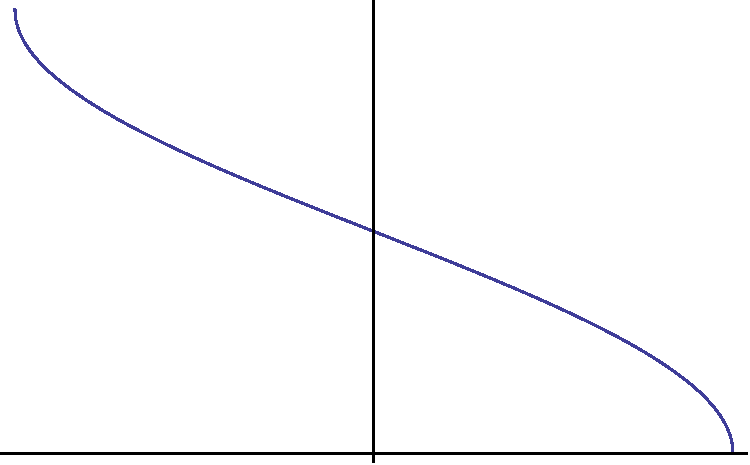
\includegraphics[width = 50 truemm]{20150422-fig-arccos.pdf} &
\begin{picture}(0,0)
\put(6,2){\dashbox{1.2}(68.3,42.3)}
\put(74.3,44.3){\dashbox{1.2}(68,42)}
\put(2,47){$-1$}
\put(140,35){$1$}
\put(76,36){$0$}
\put(75,0){$-\frac{\pi}{2}$}
\put(66,84){$\frac{\pi}{2}$}
\end{picture}
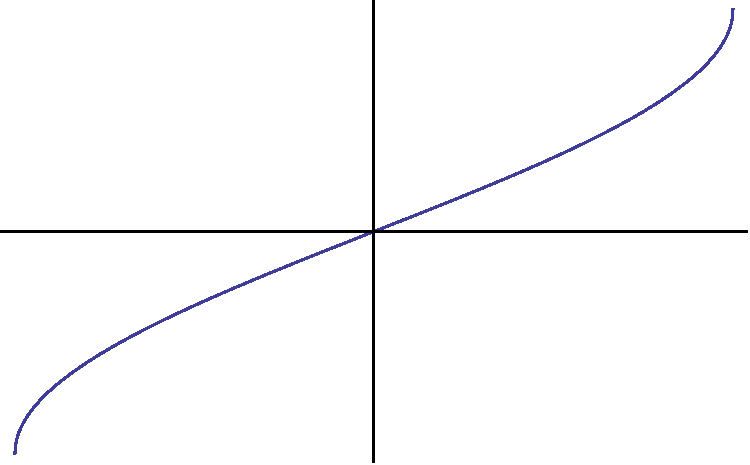
\includegraphics[width = 50 truemm]{20150422-fig-arcsin.pdf} &
\begin{picture}(0,0)
\put(2,-1){\dashbox{1.2}(72.3,0)}
\put(74.3,89){\dashbox{1.2}(72,0)}
\put(76,36){$0$}
\put(75,0){$-\frac{\pi}{2}$}
\put(66,84){$\frac{\pi}{2}$}
\end{picture}
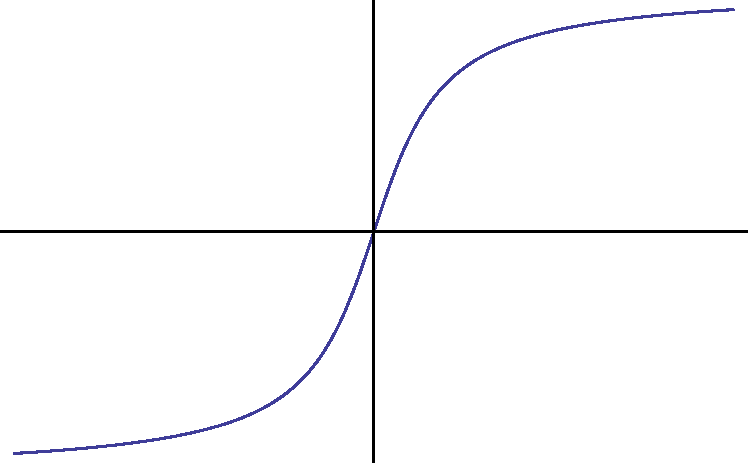
\includegraphics[width = 50 truemm]{20150422-fig-arctan.pdf} \\
$y = \arccos x$ & $y = \arcsin x$ & $y = \arctan x$
\end{tabular}
\end{center}
\end{table}

この中で一番よく使うのは$\arctan$だと思います。というのも直線$\tan$は角度から傾きを計算するのに使う函数ですから、$\arctan$は「与えられた傾きを実現する角度は何度か?」を表しています。いかにも役立ちそうですよね。

\subsection{$\arctan 1$の公式たち}

三角函数に色々な公式があるように、逆三角函数にも色々な公式があります。その中でも$\arctan$の計算公式は比較的有名です。というのも後で見るように、$\arctan$の計算ができると、$\pi/4 = \arctan 1$を使って円周率を求めることができるからです。$\arctan 1$を色々な方法で表してみましょう。

\paragraph{問2, 3の解答} $\tan$の加法定理
\[
\tan(x+y) = \frac{\tan x + \tan y}{1 - \tan x\tan y}
\]
に$u=\tan x$, $v=\tan y$を代入すると
\begin{align*}
\arctan u + \arctan v
&= x + y = \arctan \tan(x+y)
= \arctan \frac{\tan x + \tan y}{1 - \tan x\tan y}
= \arctan \Bigl(\frac{u+v}{1-uv}\Bigr)
\end{align*}
を得る。この式で$u=1/2$, $v=1/3$とおくと
\[
\arctan \frac{1}{2} + \arctan \frac{1}{3} = \arctan \Bigl(\frac{\frac{1}{2}+\frac{1}{3}}{1-\frac{1}{6}}\Bigr) = \arctan 1 = \frac{\pi}{4}
\]
が得られる。これはEulerの公式と呼ばれる。

また$u=v=1/5$とおくと、同じように計算することで
\[
2\arctan\frac{1}{5} = \arctan\frac{\frac{2}{5}}{1-\frac{1}{25}} = \arctan\frac{5}{12}
\]
となる。さらに$u=v=5/12$に対しては
\[
2\arctan\frac{5}{12} = \arctan\frac{\frac{10}{12}}{1-\frac{25}{144}} = \arctan\frac{120}{119}
\]
である。そして$u=120/119$に対し$(u+v)/(1-uv)=1$となる$v$を求めると、$v=(1-u)/(1+u)=-1/239$となる。これらをまとめると、Machinの公式
\begin{align*}
\frac{\pi}{4}
&= \arctan \frac{\frac{120}{119}+\frac{-1}{239}}{1-\frac{120}{119}\frac{-1}{239}}
= \arctan \frac{120}{119} + \arctan\frac{-1}{239}
= 2\arctan\frac{5}{12} - \arctan\frac{1}{239}
= 4\arctan\frac{1}{5} - \arctan\frac{1}{239}
\end{align*}
を得る\footnote{途中で$1$回、主値$(-\pi/2,\pi/2)$のもとで$\arctan$が奇函数であることを使います。}。 \qed

\paragraph{問4の解答} 計算自体は簡単である。
\begin{center}
\hfil (1)  $(3+i)(7+i) = 20+10i$,
\hfil (2) $(2+i)(3+i) = 5+5i$,
\hfil (3) $(5+i)^4/(239+i) = 2+2i$ \hfil
\end{center}
ただ、この問題で重要なのは計算結果から$\arctan$の公式が得られる点である。複素数$z=x+yi$の偏角が$\arctan (y/x)$で与えられること、また偏角が$\arg zz' = \arg z + \arg z'$という式を満たすことを思い出そう。両辺の偏角を取れば
\begin{align*}
\arctan\frac{1}{3} + \arctan\frac{1}{7} &= \arctan\frac{1}{2}, &
\arctan\frac{1}{2} + \arctan\frac{1}{3} &= \arctan{1} = \frac{\pi}{4},  &
4\arctan\frac{1}{5} - \arctan\frac{1}{239} &= \arctan{1} = \frac{\pi}{4}
\end{align*}
が得られる。\qed

\paragraph{問5の解答} 次の図を見れば、求める角度は直角二等辺三角形の内角だから45度と分かる。

\begin{center}
\begin{picture}(150,100)
\put(0,0){\line(1,0){150}}
\put(0,50){\line(1,0){150}}
\put(0,100){\line(1,0){150}}
\put(0,0){\line(0,1){100}}
\put(50,0){\line(0,1){100}}
\put(100,0){\line(0,1){100}}
\put(150,0){\line(0,1){100}}
\put(0,0){\line(1,2){50}}
\put(0,0){\line(3,1){150}}
\put(50,100){\line(2,-1){100}}
\put(3,13){\circle{3}}
\put(62,97){\circle{3}}
\put(45,97){\circle*{3}}
\end{picture}
\end{center}

この図もまた、$\arctan (1/2) + \arctan (1/3) = \pi/4$を表している。 \qed

\subsection{円周率の計算}

$\arctan$には、実は次のような近似公式があります:
\[
\arctan x = x - \frac{x^3}{3} + \frac{x^5}{5} - \frac{x^7}{7} + \cdots \quad \text{(if $-1\leq x\leq 1$)}
\]
この公式は、形式的には
\[
\arctan x = \int_0^x (\arctan t)' dt = \int_0^x \frac{1}{1+t^2} dt = \int_0^x (1-t^2+t^4-t^6+\cdots) dt
= x - \frac{x^3}{3} + \frac{x^5}{5} - \frac{x^7}{7} + \cdots
\]
のようにして求められます\footnote{この「証明」は全然厳密ではありません。何も考えずに無限和と積分の順序を入れ替えてはいけないからです。Taylor展開を習った後なら、こんなことをしなくても公式が導けるようになります。}。右辺は気合で頑張ればいくらでも精度よく計算できますから、この公式をガリガリ計算することで$\arctan x$の値を求めることができます。たとえば$x=1$とすれば
\[
\frac{\pi}{4} = \arctan 1 = 1 - \frac{1}{3} + \frac{1}{5} - \frac{1}{7} + \cdots
\]
という風にして円周率が求められます。これはLeibnizの公式と呼ばれているようです。

ただし、今の$\pi/4$公式は非常に効率が悪いです。というのも第$50$番目の項が$-1/99 = 0.010101\cdots$ですから、$50$番目の項を計算すると小数第$2$位の値が変わります。円周率を求める上では「ちょこっと計算しただけで、上の方の桁が正確に分かる」ような公式が望ましいわけで、こんな「$50$項も計算してもまだ小数第$2$位が分からない」なんて公式は役に立ちません。そこで登場するのがEulerの公式やMachinの公式です。たとえばEulerの公式なら
\begin{align*}
\frac{\pi}{4}
&= \arctan \frac{1}{2} + \arctan \frac{1}{3}
= \Bigl(\frac{1}{2} - \frac{1}{3\cdot 2^3} + \frac{1}{5\cdot 2^5} - \cdots\Bigr)
+ \Bigl(\frac{1}{3} - \frac{1}{3\cdot 3^3} + \frac{1}{5\cdot 3^5} - \cdots\Bigr) \\
&= \Bigl(\frac{1}{2} - \frac{1}{24} + \frac{1}{160} - \cdots\Bigr)
+ \Bigl(\frac{1}{3} - \frac{1}{81} + \frac{1}{1215} - \cdots\Bigr)
\end{align*}
のように、分母にある$x^n$の形の項が効いてきて、足し引きされる項の値が急激に小さくなっていきます。今の場合、最初から$3$つずつの項を拾うだけで$\pi=3.14\cdots$が求まります。さっきより断然楽ですね。Machinの公式に至っては$1/239$という項がありますから、少ない手間でもっと精度よい値を求められます。William Jonesという数学者が1706年に著した``Synopsis Palmariorum Mathesos''という本\footnote{ちなみに本郷キャンパスにある総合図書館の書庫内に、この本があるそうです。OPACで検索すると出てきます。}に、Machinが求めたとされる円周率が結果だけ100桁以上載っていますが、今の公式を使ったのでしょうか?

もちろん$\arctan$に放り込む数が小さくなれば小さくなるほど、計算はどんどん楽になります。したがって「$\pi$が上手く出てくる$\arctan$の公式を見つけて、君だけのオリジナルの円周率近似公式をつくろう!」…という話になりそうですが、実はこの公式は頑張ってもそんなに精度が出ません。いまの公式では分母に$x^n$が出てくることがキモだったので「$1$つ先の項を計算したときに、何桁分だけ精度が良くなるか」は毎回同じです。もし$x$が$100$だったら、次の項を考えてもせいぜい$2$桁程度しか精度が良くならないわけです。ところが世の中には「計算を$1$手進めるだけで、\textbf{それまでの桁数の倍の桁数}だけ精度が良くなる」という、圧倒的に強い公式があります。Gauss--Legendreアルゴリズムといいますので、興味のある人は調べてみてください\footnote{たとえば\href{http://www.nippyo.co.jp/book/6387.html}{四ツ谷 晶二・村井 実『楕円関数と仲良くなろう』(日本評論社)}の第$2$章に詳しい説明があります。}。

ちなみに、プリントをアップロードしているGitHubのページ\footnote{\url{https://github.com/HideakiHosaka/2015_linear_algebra}}に、Excel で円周率の近似計算の実験をした結果\texttt{pi\_approx.xlsx}を載せてみました。いくつかの公式に対し$n$番目の項の値、$n$番目の近似値と真の値からの誤差を表にしています。興味がある人は、このデータの誤差を対数プロットしてみると良いでしょう。ただしExcelは高精度計算には向かないので、途中で精度が打ち止めになっています。本気で円周率を求めるには、プログラムを書き、必要に応じて高精度計算のためのライブラリを援用しないといけません。

\section{双曲線函数と逆双曲線函数}

最後のテーマは、双曲線函数と呼ばれる函数たちです。これらは指数函数の四則演算で書けるという意味では、そこまで目新しいものではありません。ですが三角函数と良く似た性質を持ち、かつ置換積分などの際に役立つので、性質を知っておくと便利です。

\subsection{双曲線函数}

\paragraph{定義}
次に挙げる函数を、双曲線函数といいます。
\begin{align*}
\cosh x &:= \frac{e^x+e^{-x}}{2}, & \sinh x &:= \frac{e^x - e^{-x}}{2}, & \tanh x := \frac{\sinh x}{\cosh x}
\end{align*}
名前の付け方のルールは三角函数と同じです\footnote{三角函数の$\cot$, $\sec$, $\cosec$に対応して双曲線函数でも$\coth$, $\sech$, $\cosech$というのが定義されますが、使う場面はまず無いでしょう。}。

これらが双曲線函数と呼ばれる所以の一つは、双曲線のパラメータ表示を与えるからです。三角函数は$\cos^2 t + \sin^2 t =1$という恒等式を満たしましたが、双曲線函数では$\cosh^2 t - \sinh^2 t = 1$という式が成り立ちます。したがって$t$が動けば、点$(\cosh t,\sinh t)$は双曲線$x^2-y^2=1$の上を動きます。ただし$\cosh t>0$なので、このパラメータ表示は双曲線の右側だけしか与えていません。双曲線の左側のパラメータ表示は$(-\cosh t,\sinh t)$で与えられます。

他にも、双曲線を使って$\cosh$, $\sinh$に図形的方法で定義を与えることもできます。

\paragraph{問6の解答}
双曲線$u^2-v^2=1$上に、下図で塗りつぶされた部分の面積が$x/2$となるような点を取る。この点の座標を$(\cosh x, \sinh x)$と書く。$\cosh x$と$\sinh x$の明示的な式を求めよう。面積の計算には積分が必要である。積分計算を楽にするため、この双曲線を正の向き\footnote{数学でいう「正の向き」は、反時計回りです。}に$45^{\circ}$回転させる。そうすると双曲線$u^2-v^2=1$は、直線$v=u$上で原点からの距離が$1$である点、すなわち点$(\frac{1}{\sqrt{2}},\frac{1}{\sqrt{2}})$を通る反比例のグラフになる。よって回転後の双曲線の式は$\eta=\frac{1}{2\xi}$である\footnote{$\xi,\eta$はそれぞれギリシャ文字のグザイとエータです。}\footnote{軸を$u,v$から$\xi,\eta$に変えたことに、深い意味はありません。}。

\begin{figure}[h!tbp]
\begin{center}
\hfil
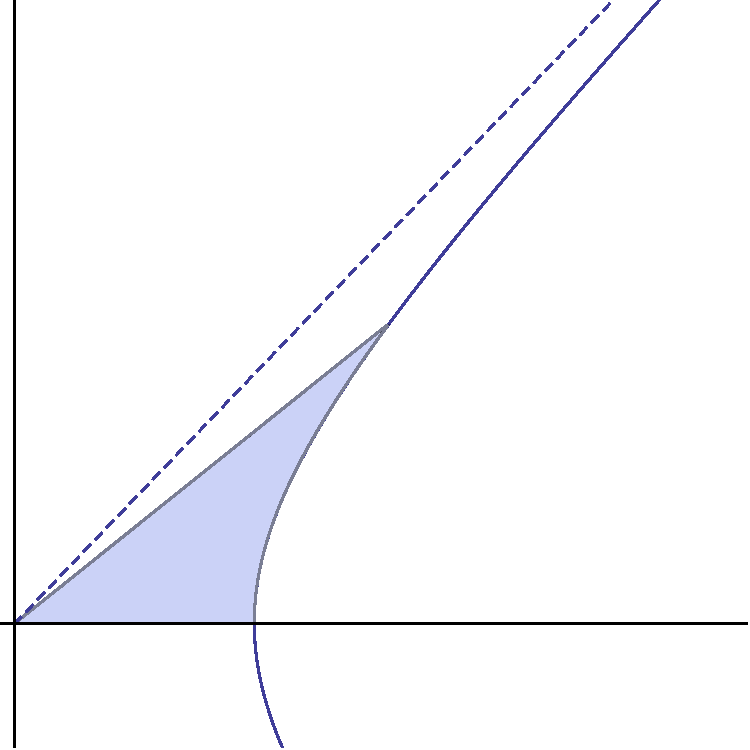
\includegraphics[width = 50 truemm, trim = 0 0  30 40, clip]{20150422-fig-hyp1.pdf}
\begin{picture}(0,0)
\put(-65,88){\circle*{3}}
\put(-64,80){$(\cosh x,\sinh x)$}
\put(-105,40){$\displaystyle \frac{x}{2}$}
\put(-40,110){$u^2-v^2=1$}
\end{picture}
 \hfil
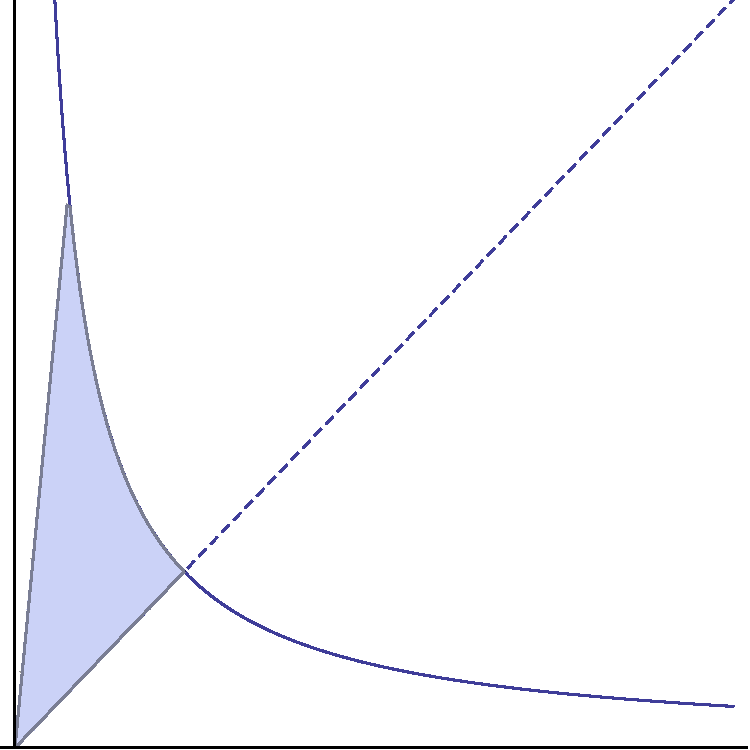
\includegraphics[width = 50 truemm, trim = 0 0 30 40, clip]{20150422-fig-hyp2.pdf}  \hfil ~
\end{center}
\end{figure}

縦より横に積分した方が見やすいので、面積を求めるべき部分を直線$\eta=\xi$について折り返す。すると、次の二つの図で示された面積は等しいことが分かる。$\mathrm{AB}\cdot\mathrm{BC} = \mathrm{PQ}\cdot\mathrm{CQ} = \frac{1}{2}$が成り立ち、$\triangle\mathrm{ABC}$と$\triangle\mathrm{CQP}$の面積が等しくなるからである。

\begin{figure}[h!tbp]
\begin{center}
\hfil
\begin{picture}(0,0)
\put(23,75){$\eta=\frac{1}{2\xi}$}
\end{picture}
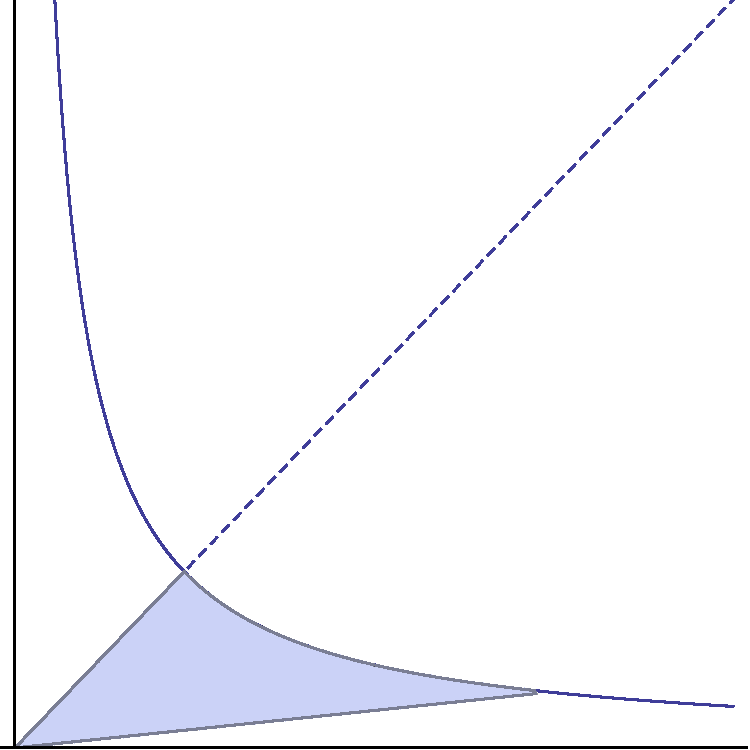
\includegraphics[width = 50 truemm,trim = 0 0 10 110, clip]{20150422-fig-hyp3.pdf} \hfil
\begin{picture}(0,0)
\put(3,-9){$\mathrm{C}$}
\put(37,-9){$\mathrm{B}$}
\put(36,39){$\mathrm{A}$}
\put(108,13){$\mathrm{P}$}
\put(98,-9){$\mathrm{Q}(\xi_0,0)$}
\put(23,75){$\eta=\frac{1}{2\xi}$}
\end{picture}
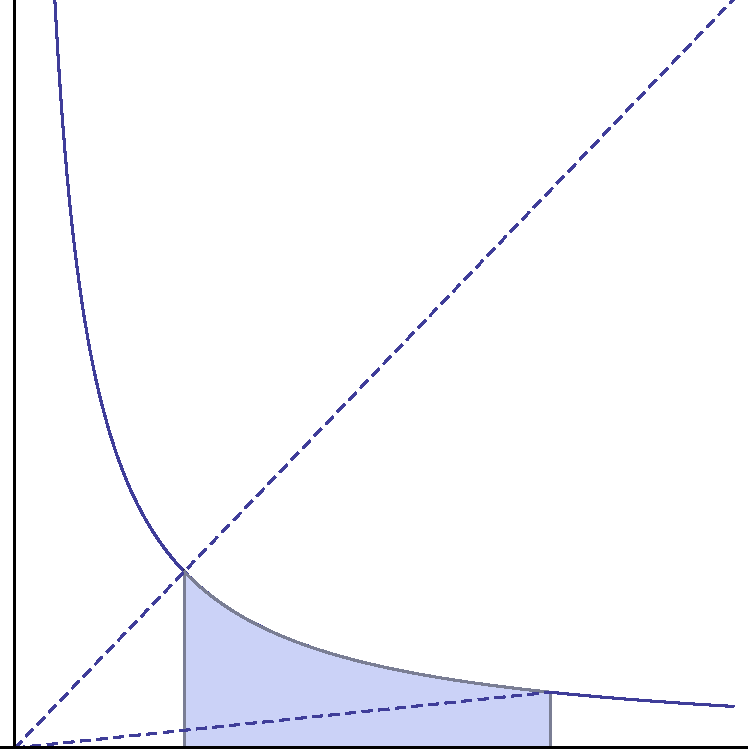
\includegraphics[width = 50 truemm,trim = 0 0 10 110, clip]{20150422-fig-hyp4.pdf}
\begin{picture}(0,0)
\put(-38.3,11){\circle*{3}}
\put(-38.3,0.5){\circle*{3}}
\put(-109.7,0.5){\circle*{3}}
\put(-109.7,35){\circle*{3}}
\put(-143,0.5){\circle*{3}}
\end{picture}
 \hfil ~
\end{center}
\end{figure}

さて点$\mathrm{Q}$の$\xi$座標を$\xi_0$とおく。$\mathrm{B}$の$\xi$座標は$\frac{1}{\sqrt{2}}$なので、積分で面積を計算すると
\[
\frac{x}{2} = \int_{\frac{1}{\sqrt{2}}}^{\xi_0} \frac{d\xi} {2\xi} = \frac{1}{2}\Bigl(\log \xi_0 - \log\frac{1}{\sqrt{2}}\Bigr)
= \frac{1}{2} \log\bigl(\sqrt{2}\xi_0\bigr)
\]
と求まる。一方で点$\mathrm{P}$は、点$(\cosh x, \sinh x)$を$x$軸について折り返してから正の向きに$45^{\circ}$度回転さることで得られるのであった。ゆえに、この平面を複素平面と同一視することで$\mathrm{P}$の座標が
\[
\overline{\cosh x + i \sinh x} \times e^{i\pi/4} = (\cosh x - i \sinh x)\Bigl(\frac{1}{\sqrt{2}} + \frac{1}{\sqrt{2}}i \Bigr)
= \frac{\cosh x + \sinh x}{\sqrt{2}} + \frac{\cosh x - \sinh x}{\sqrt{2}} i
\]
と分かる\footnote{回転行列のことを知っているなら、それを使ってももちろん同じ計算ができます。}。この実部が$\xi_0$なので、面積の計算と合わせて$x = \log (\sqrt{2}\xi_0) = \log(\cosh x + \sinh x)$が従う。つまり$\cosh x + \sinh x = e^x$である。

最後に、点$(\cosh x,\sinh x)$は双曲線$u^2-v^2=1$の上にあったことを思い出す。これより
\[
1 = \cosh^2 x - \sinh ^2 x = (\cosh x - \sinh x)(\cosh x + \sinh x) = (\cosh x - \sinh x ) e^x
\]
という式が得られる。すなわち$\cosh x - \sinh x = e^{-x}$である。かくして$\cosh x + \sinh x = e^x$と合わせて$\cosh x$と$\sinh x$の連立$1$次方程式が得られたので、これを解いて$\cosh x$と$\sinh x$の求める式を得る。 \qed

\paragraph{グラフ}  双曲線函数のグラフは次の通りです。$\cosh x$と$\sinh x$のグラフに点線で描き込まれているのは、函数$e^x / 2$と$\pm e^{-x} / 2$です。
\begin{table}[h!tbp]
\begin{center}
\begin{tabular}{ccc}
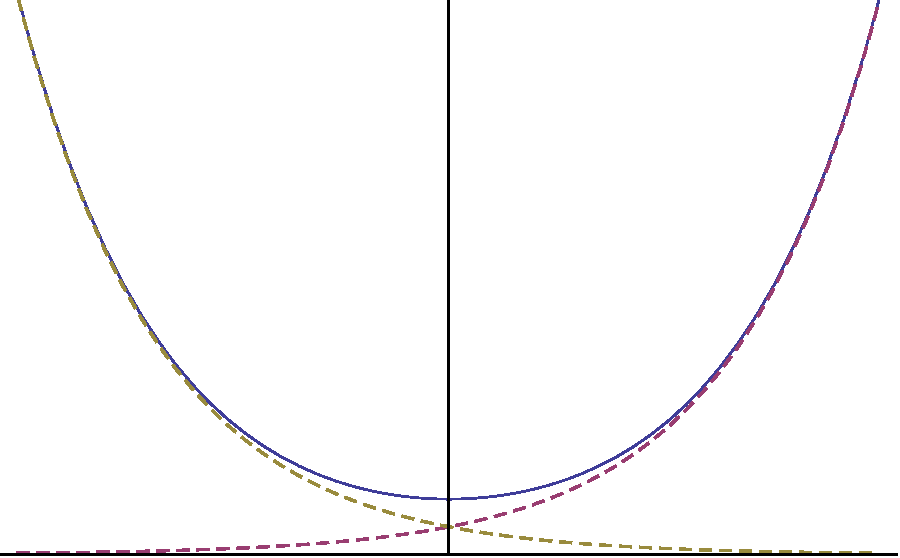
\includegraphics[width = 50 truemm]{20150422-fig-cosh.pdf} &
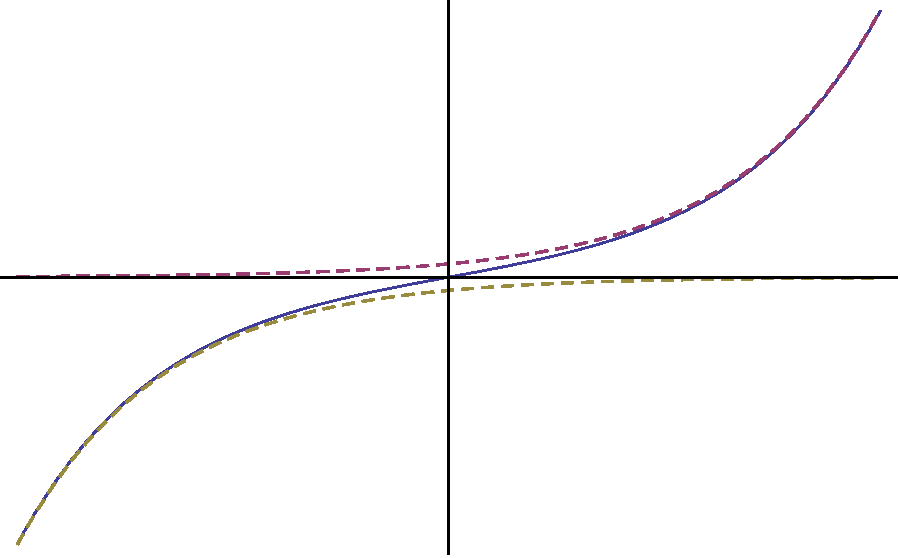
\includegraphics[width = 50 truemm]{20150422-fig-sinh.pdf} &
\begin{picture}(0,0)
\put(2,-1){\dashbox{1.2}(72.3,0)}
\put(74.3,88.5){\dashbox{1.2}(72,0)}
\put(76,36){$0$}
\put(75,-2){$-1$}
\put(66,86){$1$}
\end{picture}
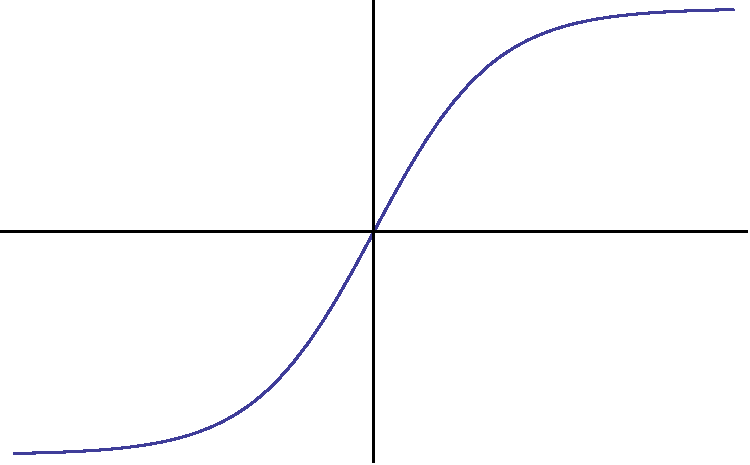
\includegraphics[width = 50 truemm]{20150422-fig-tanh.pdf} \\
$y = \cosh x$ & $y = \sinh x$ & $y = \tanh x$
\end{tabular}
\end{center}
\end{table}

本体だけ見ると$\cosh x$, $\sinh x$はそれぞれ$2$次、$3$次函数のグラフに似てなくもないです。しかし中に指数函数がいるので、$x\rightarrow\pm\infty$での絶対値の増大度が全然違います。気を付けましょう。また$\cosh x$のグラフには「懸垂線」という名前が付いています。これは、糸の両端を持ってぶら下げた時にできる曲線が$\cosh$で書けることに由来します。

\paragraph{問6 (d) の解答と導函数}
計算すると一瞬で$(\cosh x)' = \sinh x $, $(\sinh x)' = \cosh x$が分かります。これも符号の付き方が微妙に違うだけで、三角函数とよく似ています。また今の計算から、$y=\cosh x$と$y=\sinh x$は両方とも微分方程式$y''=y$の解だとが分かります。これも、単振動の方程式$y''=-y$の解が三角函数で得られることと似ています。

\paragraph{問6 (b) の解答と加法定理}
双曲線函数に関しても、三角函数と同様の加法定理が成り立ちます。ただし、符号の付き方が三角函数のときと少しだけ変わります。
\begin{align*}
\cosh x \cosh y + \sinh x \sinh y
&= \frac{e^x + e^{-x}}{2} \frac{e^y + e^{-y}}{2} + \frac{e^x - e^{-x}}{2}\frac{e^y - e^{-y}}{2} \\
&= \frac{e^{x+y} + e^{x-y} + e^{-x+y} + e^{-(x+y)}}{4} + \frac{e^{x+y} - e^{x-y} - e^{-x+y} + e^{-(x+y)}}{4} \\
&= \cosh(x+y) \\
\sinh x \cosh y + \cosh x \sinh y
&= \frac{e^x - e^{-x}}{2} \frac{e^y + e^{-y}}{2} + \frac{e^x + e^{-x}}{2}\frac{e^y - e^{-y}}{2} \\
&= \frac{e^{x+y} + e^{x-y} - e^{-x+y} - e^{-(x+y)}}{4} + \frac{e^{x+y} + e^{x-y} - e^{-x+y} - e^{-(x+y)}}{4} \\
&= \sinh(x+y)
\end{align*}

加法定理が成り立ちますから、当然ながら$n$倍角の公式や和積・積和公式の類も三角函数のやつを少し修正するだけで得られます。これらの公式は、たまに双曲線函数の掛け算を積分する際に役立ちます。大学入試のときみたいに頑張って公式を暗記する必要まではありませんが、「三角函数と同じ公式がある」ことは頭の片隅に置いておきましょう。

\paragraph{双曲線函数と三角函数の関係}

さて「三角函数と双曲線函数は似ている」ということを延々見てきたわけですが、なぜこんなにも似ているのでしょうか。それは定義域を複素数まで広げてみると分かります。前回$e^{i\theta} = \cos\theta + i \sin \theta$という式を紹介しました。そして双曲線函数は指数函数を使って定義されていますから、$e^{i\theta}$の式を使えば、双曲線函数に複素数を放り込めます。「何で指数函数に複素数を入れていいのか」は全く説明していませんが、深いことは気にしないでおきましょう。実際にやってみると
\begin{align*}
\cosh i\theta = \frac{e^{i\theta} + e^{-i\theta}}{2} &= \cos \theta, &
\sinh i\theta = \frac{e^{i\theta} - e^{-i\theta}}{2} &= i\sin \theta &
\end{align*}
というように、なんと三角函数が出てきます。つまり複素数$z\in\mathbb{C}$に対し$(e^z \pm e^{-z})/2$という函数を考えたとき\footnote{一般の複素数$z=a+i\theta$に対しては、$e^z := e^a e^{i\theta}$と定めます。}、この函数は実軸上では双曲線函数に、虚軸上では三角函数 (の$i$倍) に化けるのです。このように$\cosh$と$\cos$, $\sinh$と$\sin$の共通の親玉となる函数がいるので、似たような挙動を示していたのです。

\subsection{逆双曲線函数}

双曲線函数の逆函数を逆双曲線函数といい、三角函数の時と同様、頭に``arc''を付けて$\arccosh$などと表します。これらの函数は、$\log$と平方根で表せます。したがって微分も、今まで知っている知識だけでてできます。

\paragraph{問6 (c) の解答}

$y=\cosh x = (e^x+e^{-x})/2$とおくと、$(e^x)^2 + 1 = 2ye^x$である。よって$e^x$の$2$次方程式$(e^x)^2 - 2y e^x+1=0$を解いて
$e^x = y\pm\sqrt{y^2-1}$を得る。よって$\arccosh y = x = \log\bigl(y\pm\sqrt{y^2-1}\bigr)$である。$\pm$の符号はそれぞれ上の枝と下の枝に対応する。

同様に$y=\sinh x = (e^x - e^{-x})/2$を$e^x$について解くと$e^x=y\pm\sqrt{y^2+1}$を得る。ただし$e^x>0$なので$-$の符号は不適である。よって$x=\arcsinh x=\log\bigl(y+\sqrt{y^2+1}\bigr)$が得られる。 \qed

\paragraph{問6 (d) の解答} 地道に計算すると、次のようになる。
\begin{align*}
(\arccosh x)' &= \frac{1+\frac{2x}{2\sqrt{x^2-1}}}{x+\sqrt{x^2-1}} = \frac{1}{\sqrt{x^2-1}}, &
(\arcsinh x)' &= \frac{1+\frac{2x}{2\sqrt{x^2+1}}}{x+\sqrt{x^2+1}} = \frac{1}{\sqrt{x^2+1}}
\end{align*}
逆函数の微分法を使っても良い。$y=\cosh x$のとき$(\arccosh y)' = 1 / (\cosh x)' = 1 / \sinh x = 1 / \sqrt{y^2-1}$となる。 \qed

%(a) 点$(u_0,v_0)$を双曲線$u^2-v^2=1$上の、$u_0,v_0>0$を満たす点とする。このとき$\sinh\colon\mathbb{R}\rightarrow\mathbb{R}$は全単射だから、$v_0=\sinh t_0$となる$t_0$がただ一つ存在する。このとき$u_0^2=1+v_0^2=\cosh^2 t_0$となるので、$u_0>0$と合わせて$u_0=\cosh t_0$を得る。そして$u$軸、双曲線と直線$\mathrm{OP}$とで囲まれる部分の面積は
%\begin{align*}
%\int_0^{u_0} \frac{v_0}{u_0}u du - \int_1^{u_0} \sqrt{u^2-1} du
%&= \frac{u_0v_0}{2} - \int_0^{t_0} \sqrt{\cosh^2 t -1} \sinh t \,dt 
%= \frac{u_0v_0}{2} - \int_0^{t_0} \sinh^2 t \,dt  \\
%&= \frac{u_0v_0}{2} - \int_0^{t_0} \frac{\cosh 2t - 1}{2} \,dt
%= \frac{u_0v_0}{2} + \frac{t_0}{2} - \frac{\sinh 2t_0}{4} \\
%&= \frac{\cosh t_0 \sinh t_0}{2} + \frac{t_0}{2} - \frac{\sinh t_0 \cosh t_0}{2} = \frac{t_0}{2}
%\end{align*}
%となる。

